\documentclass[10pt]{article}
\usepackage[margin=0.95in]{geometry}
\usepackage{graphicx,amsmath,microtype,subcaption}
\usepackage[font=small]{caption}
\graphicspath{{../outputs/figures/paper/}}
\pagestyle{empty}
\setlength{\parindent}{0pt}
\setlength{\parskip}{5pt}

\begin{document}

\begin{center}
{\large\bf SHIFT-SURV: Separating Unrecoverable Information from\\
Unrecovered Performance in Multi-Center Survival Prediction}
\end{center}

\vspace{2pt}

In recent years the medical field has seen significant growth in the use of
machine-learning models for risk assessment, as they can integrate large,
multimodal data to provide personalized predictions for patients. Such models
are often trained on pooled multicenter cohorts and deployed across hospitals,
where differences in populations, measurement, treatment and outcome recording
can cause them to fail when transported to a new center. Unsupervised domain
adaptation and domain generalization are proposed as remedies, but real data
rarely reveal whether poor target performance reflects a method failure or
limited recoverability: the information the outcome depends on may not have
survived the move, in which case no method operating on the covariates could
have recovered it.

Existing benchmarks do not resolve this. Broad distribution-shift suites [1,2]
evaluate many methods across many datasets, but they report the drop in target
performance without a reference for how much of it was recoverable, and they do
not cover time-to-event outcomes, where the label is a horizon applied to a
censored process and both discrimination and calibration matter clinically. We
therefore designed a benchmark around the missing quantity rather than around
more methods or more datasets.

SHIFT-SURV generates multi-center cohorts from a latent-factor Weibull
proportional-hazards model in which the observation process is explicit, so six
shift mechanisms can be induced one at a time: covariate, measurement,
spurious-association, baseline-hazard, label-prior and concept shift. Each
center draws invariant and spurious latent factors, and a regime perturbs
exactly one element of the pipeline while the rest is inherited, so the cause of
any degradation is known by construction. Methods are compared against
empirical risk minimization and against two analytic references. The
latent-feature reference is fitted on the true invariant factors, which no
deployed model observes. The target-data oracle is fitted on the target's own
covariates using target labels, and states how well the outcome could be
predicted from the information actually available there. The gap between ERM and
that oracle is the recoverable margin; the gap between the two references is
information the observation process did not preserve. Configurations are
calibrated so that class balance and baseline discrimination match the ranges
observed across real centers, and a margin of $0.02$ AUROC is fixed in advance
as the smallest difference treated as clinically relevant.

\begin{figure}[t]
\centering
\begin{subfigure}[t]{0.49\textwidth}
  \centering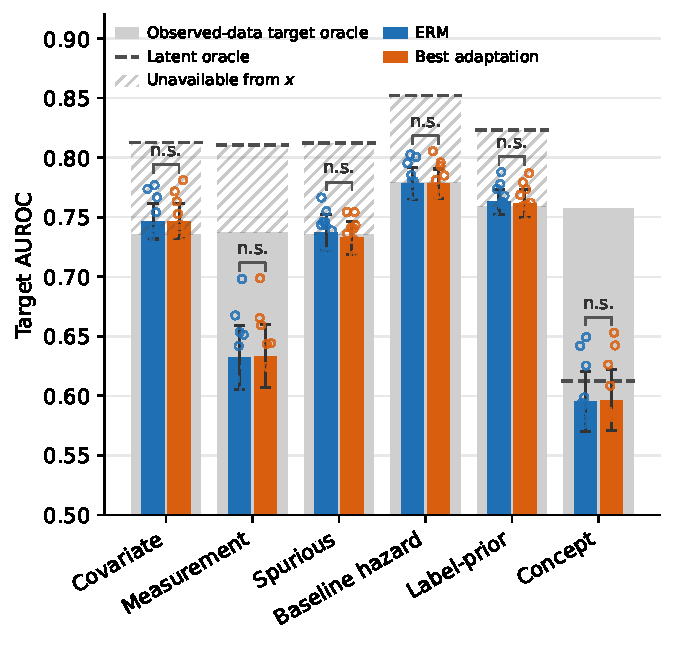
\includegraphics[width=\linewidth]{fig_disc_a.pdf}
  \caption{Discrimination}
\end{subfigure}\hfill
\begin{subfigure}[t]{0.49\textwidth}
  \centering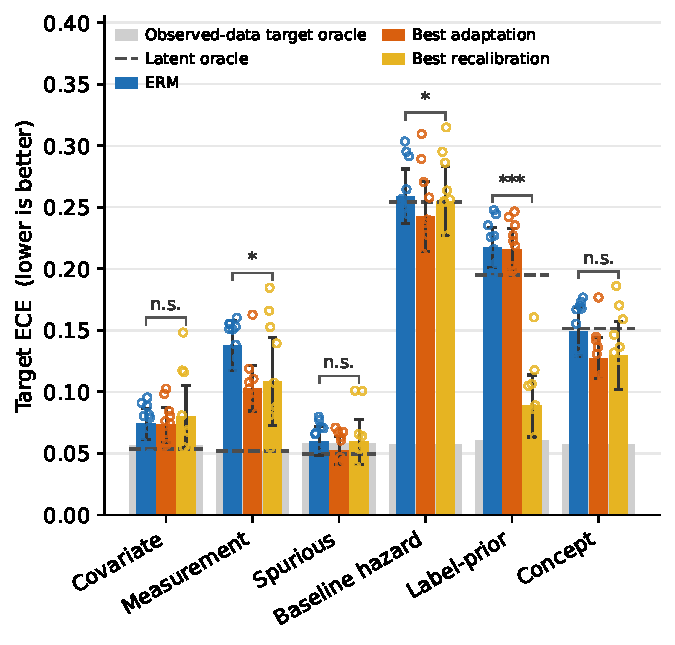
\includegraphics[width=\linewidth]{fig_cal_a.pdf}
  \caption{Calibration}
\end{subfigure}
\caption{Target performance per shift regime under the adaptation protocol. Grey
bars are the target-data oracle, the performance the target's own covariates
support; dashed rules are the latent-feature reference. The distance a method is
responsible for is its distance from the grey bar, not from the dashed rule.}
\end{figure}

The recoverable margin turns out to be near zero in four of the six regimes:
ERM already reaches what the target covariates support, so a negative result
there carries little information about adaptation. Two regimes leave room, and
neither is closed. Under measurement shift the margin is $0.105$ AUROC and the
best of IW-ERM, CORAL, DANN and CDAN recovers $0.001$ of it; under concept shift
the margin is $0.163$ and the best method recovers $0.003$. Across all regimes
the largest mean gain over ERM is $+0.003$, and an exact sign-flip permutation
test on the studentized maximum across methods returns no $p$ below $0.47$.
Calibration responds to the same shifts differently: three regimes improve
significantly, and prior adjustment [3] under label-prior shift, the one pairing
in which a method's assumption matches the mechanism, reduces calibration error
from $0.217$ to $0.088$ against an oracle floor of $0.060$. No single strategy
improves both properties.

The pattern holds outside the simulator. On the I3LUNG non-small-cell lung
cancer cohort ($n=2074$, six centers) and a public breast cancer registry, no
method improves discrimination over ERM, and even a summary that selects the
best method separately for each target cohort has an upper $95\%$ limit of
$+0.006$, a quarter of the pre-specified margin. A sensitivity analysis over
$1392$ generator configurations, with every apparent counterexample re-run on
disjoint seeds, produces no adaptation gain that survives confirmation.

SHIFT-SURV is released as a configurable generator with the shift mechanisms,
the two references and the evaluation protocol. Its contribution is not another
comparison of methods but a way to ask whether a comparison is informative at
all: a transfer drop reported without a recoverability reference cannot
distinguish a method failure from an impossibility.

\vspace{4pt}
{\footnotesize
[1] P. W. Koh et al. \emph{WILDS: A benchmark of in-the-wild distribution
shifts.} ICML, 2021.\\
[2] I. Gulrajani and D. Lopez-Paz. \emph{In search of lost domain
generalization.} ICLR, 2021.\\
[3] M. Saerens, P. Latinne and C. Decaestecker. \emph{Adjusting the outputs of a
classifier to new a priori probabilities.} Neural Computation, 14(1),
21--41, 2002.\\
[4] A. Prelaj et al. \emph{I3LUNG: Clinical validation of a multimodal AI tool
to support immunotherapy decisions in NSCLC.} medRxiv, 2026.
}

\end{document}
